\section{System Overview}
\subsection{Brief Introduction of System Function}
With the increasing popularity of network technology and the importance of information construction, people increasingly need a file synchronisation tool to help them get the file they want on different devices. File synchronisation tools make it possible to edit the same files across multiple computers in a sensible way. This system is a ‘hub and spoke’ file synchroniser which have a single central server (the ‘hub’) to which multiple other clients (the ‘spokes’) synchronise. Developing such a tool can bring a lot of convenience to the users as it can let them get the files they need, anytime, anywhere.\\\\
Therefore, our team, \emph{Deadline Fighters}, are aims to develop a multi-host file synchronizer which can:
\begin{itemize}
\item{Allow upload and download of files from a central server (hub) through client applications with necessary authorization.}
\item{Automatically synchronize changes made by client applications unto the corresponding copy of the file in the server.}
\item{Handle all possible conflict/non-conflict scenarios of file synchronization (ie. combinations of Create, Edit, Rename, Delete) involving multiple client applications.}
\item{Enable file synchronisation through both desktop (all platform) and mobile (Android) clients.}
\end{itemize}
as we set in the initial report.\\\\
Through the outline of initial report, we detailed each function. Therefore, the file synchronisation tool that our team aim to develop will achieve the following functions as designed during the process: Upload a file from local which is outside the local sync folder; Upload files from local sync folder; Download a file from server; Download files from server; Delete a file/files from local sync folder; Delete a file/files from server; Rename a file/two or more files from local sync folder; Rename a file/two or more files from server; List all files on the server; Edit a file from server; Edit two or more files from server; Synchronize server and local files.\\\
What’s more, the file synchronisation tool can be used in both desktop (all platform) and mobile (Android) clients.\\\\
\begin{table}[H]
\caption{Priority of operations}
\centering
\begin{tabular}{|c|p{2cm}|c|p{3cm}|}
\hline
Operation & Object & Priority & Description \\
\hline
\multirow{2}{*}{Upload}&{One file (May not in the local sync folder)}&1&{Priority description:}\\
\cline{2-3}
&All files in the local sync folder&2&{1. Functions Necessary and Important}\\
\cline{1-3}
\multirow{2}{*}{Download}&{One file}&1&{2. Characteristic Functions}\\
\cline{2-3}
&All files&2&{3. General functions}\\
\cline{1-3}
\multirow{2}{*}{Delete}&{One file}&2&{4. Functions can be supplemented}\\
\cline{2-3}
&All files&3&{5. Additional functions}\\
\cline{1-3}
\multirow{2}{*}{Rename}&{One file}&2&{}\\
\cline{2-3}
&Two or more files&3&{}\\
\cline{1-3}
\multirow{2}{*}{Edit}&{One file}&4&{}\\
\cline{2-3}
&Two or more files&4&{}\\
\cline{1-3}
\multirow{1}{*}{Synchronize}&{All files in the server and local syn folder}&2&{}\\
\cline{1-4}
\bottomrule
\end{tabular}
\end{table}

\subsection{System user role}
There are two types of clients using file synchronisation tools, desktop client (all platform) and mobile client (Android).\\\\
Desktop (all platform) clients:

\begin{table}[H]
\centering
\caption{Desktop (all platform) client role}
\begin{tabular}{|c|c|}
\hline
Client name & User role\\
\hline
{Desktop (all platform)} & View files on the server \\ \cline{2-2}
& Upload a file from local which is outside the local sync folder \\
\cline{2-2}
& Upload files from local sync folder\\
\cline{2-2}
&Download a file/files from server\\
\cline{2-2}
&Delete a file from local sync folder\\
\cline{2-2}
&Delete a file from server\\
\cline{2-2}
&Rename a file from local sync folder\\
\cline{2-2}
&Rename a file from server\\
\cline{2-2}
&Edit a file from server\\
\cline{2-2}
&Edit two or more files from server\\
\cline{2-2}
&Synchronize server and local files\\
\hline
\bottomrule
\end{tabular}
\end{table}


\begin{table}[H]
\centering
\caption{Mobile (Android) client role}
\begin{tabular}{|c|l|}
\hline
Client name & User role\\
\hline
{Mobile (Android)} & View files on the server \\ \cline{2-2}
& Upload a file from local which is outside the local sync folder \\
\cline{2-2}
& Upload files from local sync folder\\
\cline{2-2}
&Download a file/files from server\\
\cline{2-2}
&Delete a file from local sync folder\\
\cline{2-2}
&Delete a file from server\\
\cline{2-2}
&Rename a file from local sync folder\\
\cline{2-2}
&Rename a file from server\\
\cline{2-2}
&Edit a file from server\\
\cline{2-2}
&Edit two or more files from server\\
\cline{2-2}
&Synchronize server and local files\\
\hline
\bottomrule
\end{tabular}
\end{table}

\subsection{Central server’s conflict role}
For central server: it will solve the conflict between multiple users operate at same time. The operate and resolution is shown as follow table.\\\\
(Add conflict table here.)\\\\
By using the conflict role as above in the file synchronisation tool development allows the system to reduce the number of error reports and make the system organized. It won't cause the system to lose files and report error when the user using two different synchronization functions at the same time to the server (eg. A client edit a file on the desktop application and the client delete the file on the mobile at the same time). It can avoid unnecessary data losses. Because the most important thing about a synchronous system is that you can't lose files. Through the table listed above, our team group can have a common standard for dealing with conflicts in the development process, making the development process more organized.\\\\
According to the above detailed requirements design and contradictory solutions, it can help our team have a better assignment for the tasks to the team members and promote the teamwork. Team members can arrange their own time according to their own tasks to complete system functions implementation.\\\\

\section{User Scenario}
\subsection{User Overall Scenario Description}

\begin{table}[H]
\centering
\caption{User Overall Scenario Description}
\begin{tabular}{|c|c|c|}
\hline
Role & Need & Scenario\\
\hline
{Users} & View & Files on the server \\
\cline{2-3}
& Upload  & A file from local which is outside the local sync folder \\
\cline{3-3}
& {} & Files from local sync folder\\
\cline{2-3}
&Download & A file/files from server\\
\cline{2-3}
&Delete & A file from local sync folder\\
\cline{3-3}
&{} & A file from server\\
\cline{2-3}
&Rename & A file from local sync folder\\
\cline{3-3}
&{} & A file from server\\
\cline{2-3}
&Edit & A file from server\\
\cline{3-3}
&{} & Two or more files from server\\
\cline{2-3}
&Synchronize & Files in server and local\\
\hline
\bottomrule
\end{tabular}
\end{table}

User use case:\\
\begin{minipage}
\centering
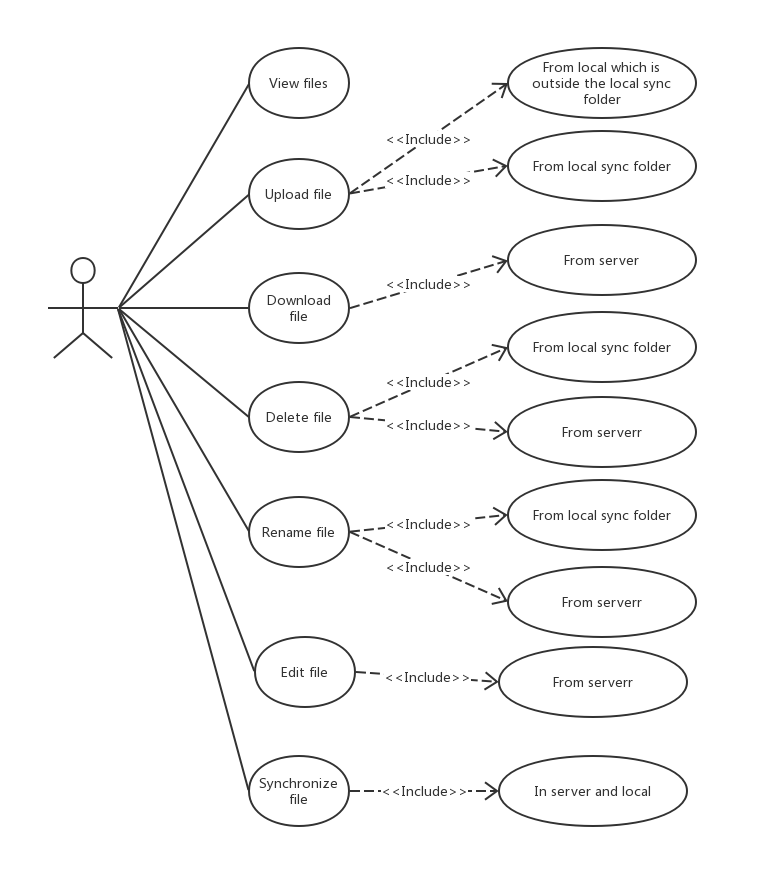
\includegraphics[scale=0.5]{User_use_case.png}

\label{fig:User use case}
\end{minipage}

\subsection{User Sub-scenario Description}
Scenario 1 View files on the server\\\\
Scenario 2 Upload a file from local which is outside the local sync folder\\\\
